%% Chapter 4 : Model for PV Energy Evaluation

\section{Air Mass Ratio}
\
\
\
\
Solar radiation has to pass through the earth's atmosphere to reach the surface. The atmosphere consists of various components which absorb a part of the solar radiation, hence reducing the solar radiation reaching the earth's surface. Moreover, longer the path the solar radiation takes through the atmosphere, more is the absorption and eventually more is the reduction in the amount of radiation reaching the surface.

\begin{figure}[H]
\centering
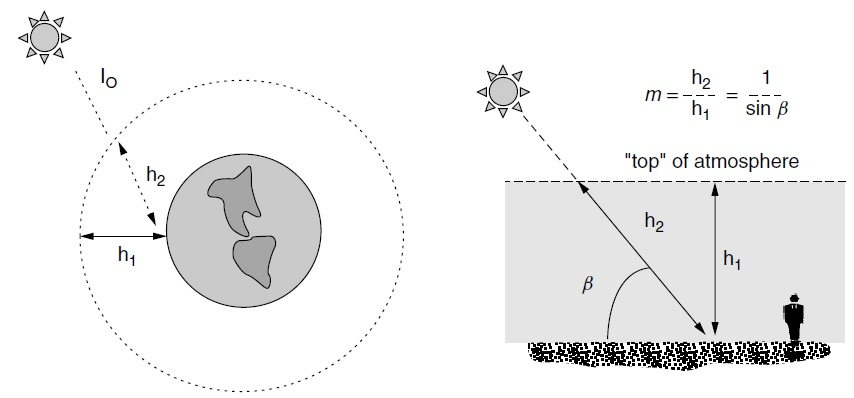
\includegraphics[scale=0.5]{m1}
\caption{The Air Mass Ratio is a measure of the amount of atmosphere the Sun's rays must pass through to reach Earth's surface [5]}
\label{figc3h1} %% to refer use, \ref{}
\end{figure}

From the Fig (\ref{figc3h1}) we say that the air mass ratio is the ratio of the actual distance h_{2} taken by the radiation through the atmosphere to reach the surface and the shortest distance h_{1} when the sun is directly overhead, with an additional assumption that the earth's surface is flat. The eq (\ref{amr}) give the air mass ratio formula.

\begin{equation}
\label{amr}
\text{Air Mass Ratio}\quad m=\frac{h_{2}}{h_{1}}=\frac{1}{•\sin{\beta}}
\end{equation}\\
where,\\
$ m $ = Air Mass Ratio \\
$ \beta $ = Altitude angle of the Sun $ (Degrees) $ \\

\section{Earth's Orbit}
\
\
\
\
Earth revolves around the sun in an elliptical orbit, as the eccentricity of this orbit is small the orbit is fairly circular. However, the distance of the earth from the sun varies everyday, with the furthest distance being when earth is at the aphelion and the shortest distance being when earth is at the perihelion. The Fig (\ref{figc4h2}) illusrates this variation in the distance of earth from the sun. We see that the summer solstice and the winter solstice happen at the aphelion and perihelion respectively; whereas the equinoxes happen visually in the midway between aphelion and perihelion.

\begin{figure}[H]
\centering
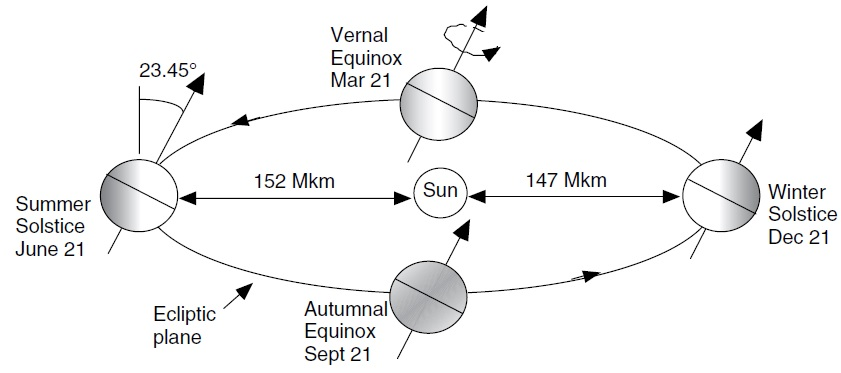
\includegraphics[scale=0.5]{m2}
\caption{Tilt of the Earth's Axis with respect to the Ecliptic Plane [5]}
\label{figc4h2} %% to refer use, \ref{}
\end{figure}

The eq (\ref{eo}) gives the variation of earth's distance from the sun.

\begin{equation}
\label{eo}
d=1.5\times10^{8}\left \{\ 1+0.017 \sin \left[ \frac{360(n-93)}{365} \right] \right\} \ \text{km}
\end{equation}\\
where,\\
$ d $ = Distance of Earth from Sun $ (km) $\\ 
$ n $ = Julian day number\\


\section{Solar Declination}
\
\
\
\
Earth revolves around the sun in an elliptical orbit with its north-south axis tilted at an angle of 23.45^{\circ}; this causes the apparent movement of the sun in the day sky to be the highest during the summers in the northern-hemisphere and lowest during the winters. Hence, the sun reaches the highest point in the sky on summer solstice (21^{st} June) when it is directly overhead the Tropic of cancer at latitude 23.45^{\circ}, and it is at the lowest point on the winter solstice (21^{st} December) when it is directly overhead the Tropic of Capricorn at the latitude 23.45^{\circ} below the equator. Moreover on both the vernal (21^{st} March) and autumnal (21^{st} September) equinox the sun is directly overhead the equator at latitude 0^{\circ}. The Fig (\ref{figc4h3}) illustrates this apparent movement of the sun in the day sky. 

\begin{figure}[H]
\centering
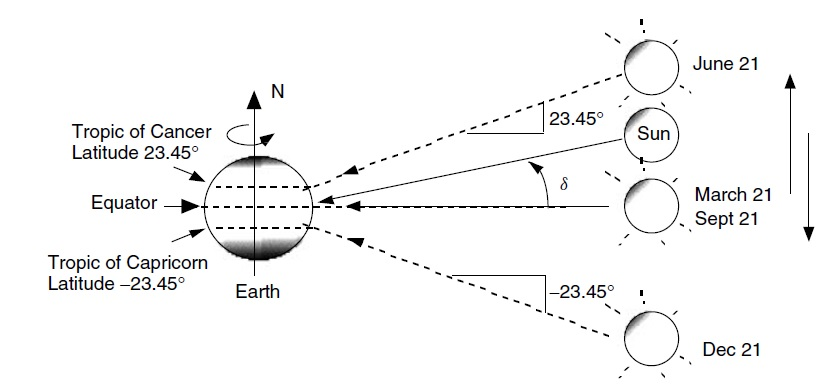
\includegraphics[scale=0.5]{m3}
\caption{The angle between Sun and Equator is called Solar Declination [5]}
\label{figc4h3} %% to refer use, \ref{}
\end{figure}

Hence, the angle formed between the plane of the equator and the line drawn from the center of the sun to the earth's center is called the solar declination angle, which is given by eq (\ref{sdec}).

\begin{equation}
\label{sdec}
\delta =23.45 \sin \left[ \frac{360}{365} (n-81)\right]  
\end{equation}\\
where,\\
$ \delta $ = Declination angle $ (Degrees) $\\

\begin{figure}[H]
\centering
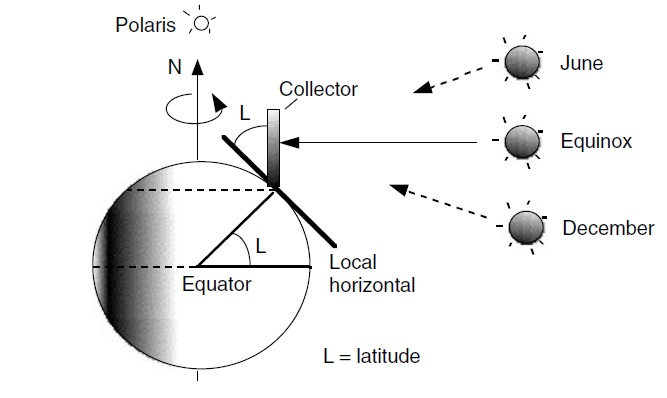
\includegraphics[scale=0.5]{m4}
\caption{A south-facing collector tipped up to an angle equal to its latitude is perpendicular to the Sun's rays at noon during Equinoxes [5]}
\label{figc4h4} %% to refer use, \ref{}
\end{figure}

The Fig (\ref{sdec}) shows the utilization of the solar declination angle in setting up the tilt of a solar panel for maximum energy output. It can be seen that, if the PV module located at a particular latitude is given a tilt equal to the tilt of the latitude the sun would be directly overhead the PV module on the equinoxes giving the best annual energy output performance for a fixed tilt PV module system.

\newpage

\section{Sun's Position}
\
\
\
\
The position of the sun in the sky is described using two angles: the azimuth and the altitude angle. The azimuth angle by convention is the angle made by the with respect to the south, being positive in the eastern direction and negative in the western direction. The altitude angle is angle made by the sun as measured positively from the earth's surface to its vertical position in the sky. The Fig (\ref{figc4h7}) illustrates the azimuth and altitude angles clearly.

\begin{figure}[H]
\centering
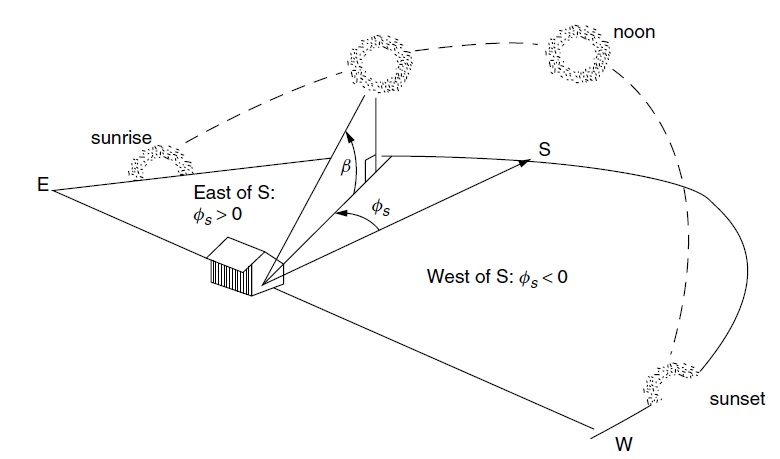
\includegraphics[scale=0.5]{m7}
\caption{Sun's Position described by its Altitude angle and Azimuth angle [5]}
\label{figc4h7} %% to refer use, \ref{}
\end{figure}

The eq (\ref{alt},\ref{azm}) give the formulas for the altitude and azimuth angles, it can be seen that they are functions of the latitude, the hour angle and the solar declination.

\begin{equation}
\label{alt}
\sin{(\beta)}=\cos{(L)}\cos{(\delta)}cos{(H)}+\sin{(L)}\sin{(\delta)}
\end{equation}\\
where,\\
$ \beta  $ = Altitude Angle $ (Degrees) $\\
$ H $ = Hour Angle $ (Degrees) $\\

\begin{equation}
\label{azm}
\sin{(\phi_{S})}=\frac{\cos{(\delta)}\sin{(H)}}{\cos{(\beta)}}
\end{equation}\\
where,\\
$ \phi_{S}  $ = Azimuth Angle of Sun $ (Degrees) $\\

The Fig (\ref{figc4h9}) illustrates the concept of the hour angle. It is the number of degrees that the earth rotates before the sun is directly overhead the local meridian (line of longitude passing through the location). So, the hour angle can also be defined as the difference between the local and the sun's meridian; it is positive till the point the sun crosses the local meridian ,and then on negative.

\begin{figure}[H]
\centering
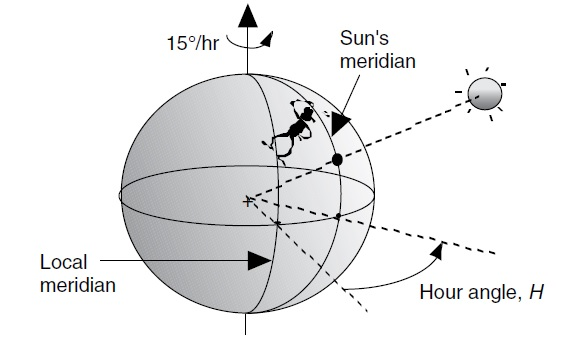
\includegraphics[scale=0.5]{m8}
\caption{The Hour angle is he number of degrees the Earth must turn before the sun is directly over the local meridian [5]}
\label{figc4h9} %% to refer use, \ref{}
\end{figure}

The eq (\ref{ha}) gives the formula for the hour angle. The factor $ \frac{15^{\circ}}{\text{hour}} $ appears as the earth takes one hour to rotate through 15^{\circ}. 

\begin{equation}
\label{ha}
\text{Hour Angle}\ H=\left(\frac{15^{\circ}}{\text{hour}}\right).(\text{hours before solar noon})
\end{equation}

The eq (\ref{hac}) provides the necessary condition for determining if th azimuth is greater or lesser than 90^{\circ} away from the south. This condition has to be applied because during spring and summer in the early morning and late afternoon the magnitude of sun's azimuth is liable to be more than 90^{\circ}; which would eventually cause the ambiguous nature of the inverse sine in eq (\ref{azm})to manifest itself.

\begin{equation}
\label{hac}
\text{if,} \quad \cos{(H)}\geq\frac{\tan{(\delta)}}{\tan{(L)}}; \hspace{1cm} \text{then,} \ |\phi_{S}|\leq90^{\circ}; \hspace{1cm} \text{otherwise,} \ |\phi_{S}|>90^{\circ}
\end{equation}

\begin{figure}[H]
\centering
\includegraphics[scale=0.5]{SunPath1}
\caption{Sun Path Diagram generated by the Sun Path Diagram App}
\label{figc4h8} %% to refer use, \ref{}
\end{figure}

The Fig (\ref{figc4h8}) shows the output of the Sun Path Diagram App developed, for the Julian Day of 100 at 30^{\circ} latitude at a resolution of 5 minutes. The red and blue curves show the summer and winter soltice sun paths, whereas the green curve shows the sun path during the two equinoxes, and the black curve shows the sun path for the 100^{th} Julian Day.

\newpage

\section{Relationship Between Solar Time and Civil Time}

The Solar Time (ST) is the time, where everything is measured relative to the solar noon at the longitude of the location, whereas the  Civil Time (CT) is the time, where everything is measured relative to the solar noon at the longitude of the regional time zone. In order to have a connection between the ST and CT two adjustments : Longitude adjustment and Equation of time adjustment, have to be done.\\

The Longitude correction involves the time taken by the sun to travel between the regional time meridian and the location time meridian. It takes 4 minutes for the sun to pass through 1^{\circ} of longitude due to the earth's rotation. Hence the factor of $ \frac{4 \ \text{min}}{\text{degree}} $ is seen in the eq (\ref{solartime}).\\

The Equation of time adjustment is required due to the earth's ellipticl orbit around the sun, which causes the length of the solar day (Solar noon to solar noon) to vary throughout the year. The Fig (\ref{figc4h10}) shows the variation in the length of the solar day throughout the year.

\begin{figure}[H]
\centering
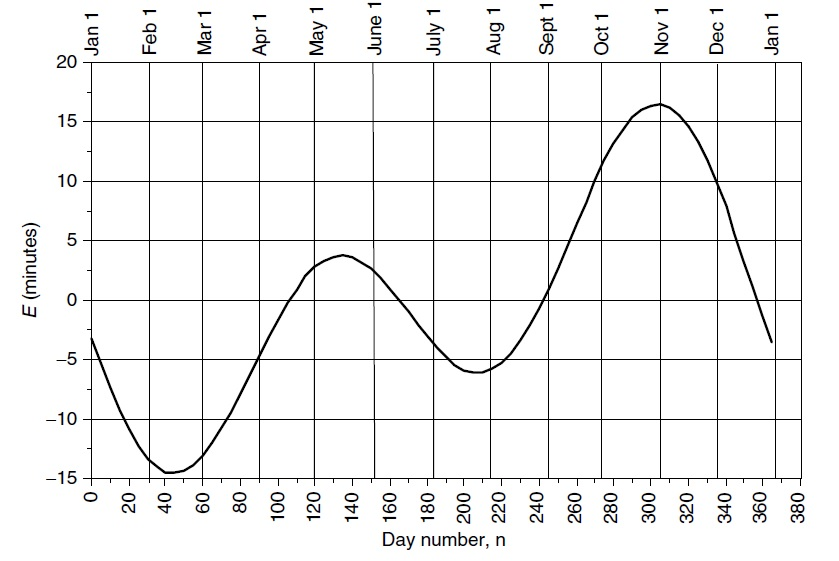
\includegraphics[scale=0.5]{m10}
\caption{The Equation of Time plotted for all year days [5]}
\label{figc4h10} %% to refer use, \ref{}
\end{figure}

The eq (\ref{eot}) give the expression for calculating equation of time.

\begin{equation}
\label{eot}
E= 9.87\sin{(2B)} -7.53\cos{(B)} -1.5\sin{(B)} \quad \text{minutes}
\end{equation}

\begin{equation}
\label{eotb}
B=\frac{360}{364}(n-81)
\end{equation}\\
where,\\
$ E $ = Equation of Time $ (mins) $ \\
$ B $ = Equation of Time angle $ (Degrees) $ 

Finally, combining everything together we get the connection between the ST and CT whic is given by the eq (\ref{solartime}).

\begin{equation}
\label{solartime}
\text{Solar Time (ST)}= \text{Clock Time (CT)}+ \frac{4 \ \text{min}}{\text{degree}}(\text{Local Time Meridian}- \text{Local Logitude})^{\circ} + E(\text{min})
\end{equation}

\subsection{Sunrise and Sunset Times}
\
\
\
\
The eq (\ref{alt},\ref{azm}) can be used to calculate the sun rise and sun set times approximately. These equations are solve for the hour angle  by putting \beta = 0 (since altitude angle of the sun during sun rise and set is zero) as seen in eq (\ref{sunrise1},\ref{sunrise2}),    
    
\begin{equation}
\label{sunrise1}
\sin{(\beta)}=\cos{(L)}\cos{(\delta)}cos{(H)}+\sin{(L)}\sin{(\delta)}=0
\end{equation}

\begin{equation}
\label{sunrise2}
\cos{(H)}=-\frac{\sin{(L)}\sin{(\delta)}}{\cos{(L)}\cos{(\delta)}}=-\tan{(L)}\tan{(\delta)}
\end{equation}

Hence, solving for the hour angle we get eq (\ref{sunrise3}).

\begin{equation}
\label{sunrise3}
H_{SR}=\cos^{-1}{(-\tan{(L)}\tan{(\delta)})} \quad \text{(+ for sunrise)}
\end{equation}

As we have see that the earth rotates $ 15^{\circ}/h $, we get the geometric sunrise time from the eq (\ref{sunrise4}). 

\begin{equation}
\label{sunrise4}
\text{Sunrise(geometric)}= 12:00-\frac{H_{SR}}{15^{\circ}/h}
\end{equation}

The geometric sun rise time refers to the point in time when the sun's center has crossed the horizon, which makes it inaccurate. Moreover, the the refraction caused by the atmosphere causes the sun to appear to rise about 2.4 minutes earlier than the geometric sun rise time and set 2.4 minutes later. Also, the definition of sun rise and sun set according to the weather services is the time when the upper limb of the sun crosses the horizon, but for us it is the crossing of the sun's center across the horizon. Futhermore, this is complicated even more by the fact that the sun rises and sets quicker around equinoxes than around the solstices due to the additional sideward movement the the later periods. Hence, in order to adjust to all these factors an adjustment factor called Q is given by the U.S. Department of Energy in 1978, its expression is given in eq (\ref{sunrise5}).

\begin{equation}
\label{sunrise5}
Q=\frac{3.467}{\cos{(L)}\cos{(\delta)}\sin{(H_{SR})}} \quad (\text{min})
\end{equation}\\
where,\\
$ Q $ = Adjustment factor $ (mins) $ \\
    
\newpage
    
\section{Types of Radiation}
\
\
\
\
The solar radiation striking the solar collector (PV modules) consists of three components. The first one is the direct-beam radiation, it is the part of solar radiation which passes in a straight line through the atmosphere to the solar collector. The second is the diffuse radiation, it the part of solar radiation which is scattered by the molecules and aerosols. Finally the last one is the reflected radiation, it is the part of solar radiation which gets reflected from the ground surface onto the solar collectors surface. The Fig (\ref{figc4h11}) illustrates the three components of solar radiation which are impressed on the solar collectors surface.\\

Note: All the equations henceforth for solar radiation were developed by Threkeld and Jordan (1958), these equations are used in the AHRAE Clear-Day Solar Flux Model.

\begin{figure}[H]
\centering
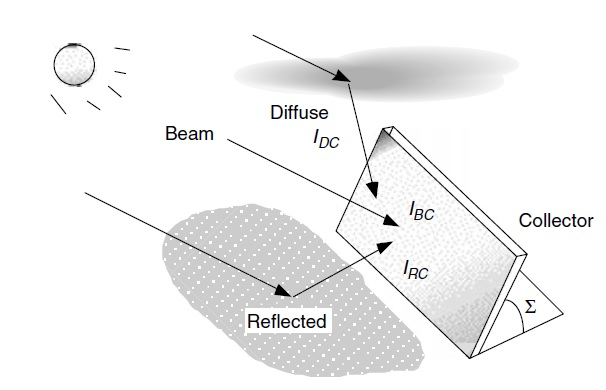
\includegraphics[scale=0.5]{m11}
\caption{Solar radiation striking a collector is a combination of Direct Beam, Diffuse and Reflected radiations [5]}
\label{figc4h11} %% to refer use, \ref{}
\end{figure}

The Fig (\ref{figc4h12}) shows the extra-terrestrial solar insolation, which is the the solar radiation passing perpendicularly through an imaginary surface just outside earth's surface.

\begin{figure}[H]
\centering
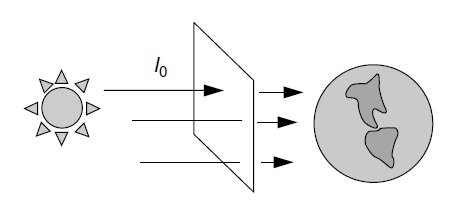
\includegraphics[scale=1]{m12}
\caption{Extraterrestrial Solar Flux [5]}
\label{figc4h12} %% to refer use, \ref{}
\end{figure}

The eq (\ref{etr1}) gives the expression for the extra-terrestrial solar insolation.

\begin{equation}
\label{etr1}
I_{0}=\text{SC}. \left[1+0.0334\cos\left(\frac{360n}{365}\right)\right] \quad (\text{W/m}^{2})
\end{equation}\\
where,\\
$ I_{0} $ = Extra Terrestrial Solar Insolation $ (W/m^{2}) $ \\
$ SC $ = Solar constant $ (1.353 kW/m^{2}) $ \\

\subsection{Beam Radiation}
\
\
\
\
The earth's atmosphere with its mixture of gases and man made aerosols causes the attenuation of the beam radiation passing through it due to absorption. The attenuation can be quantified approximately using the exponential decal function as given in the eq (\ref{beam1}).
    
\begin{equation}
\label{beam1}
I_{B}=Ae^{-km}
\end{equation}\\
where,\\
$ I_{B} $ = Beam portion of the radiation $ (W/m^{2})$\\
$ A $ = Apparent Extra-Terrestrial Flux $ (kW/m^{2})$\\
$ k $ = Optical depth \\

A given in eq (\ref{beam2}) is the apparent extra-terrestrial insolation, k given in eq (\ref{beam3}) is a dimenionless quantity called the optical depth and m is the air mass ratio as computed in eq (\ref{amr}).

\begin{equation}
\label{beam2}
A=1160+75\sin\left[\frac{360}{365}(n-275)\right] \quad (\text{W/m}^{2})
\end{equation}

\begin{equation}
\label{beam3}
k=0.174+0.035\sin\left[\frac{360}{365}(n-100)\right]
\end{equation}

The Fig (\ref{figc4h13}) illustrayes the direct beam radiation incident on a solar collector.
    
\begin{figure}[H]
\centering
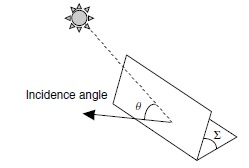
\includegraphics[scale=1]{m14}
\caption{Incidence angle between Sun and normal to the collector surface [5]}
\label{figc4h13} %% to refer use, \ref{}
\end{figure}

The component of direct beam radiation striking the surface of the solar collector is given by the eq (\ref{beamc1}).

\begin{equation}
\label{beamc1}
I_{BC}=I_{B}\cos{(\theta)}
\end{equation}\\
where,\\
$ I_{BC} $ = Beam radiation normal to the surface of the collector $ (W/m^{2})$\\
$ \theta $ = Angle between a line drawn normal to the solar collector face and the incoming beam
radiation $ (Degrees)$\\

The Fig (\ref{figc4h14) shows a complicated geometry of a solar collector, which has a tilt angle and an azimuth angle. The computation of the incidence angle of this solar collector is done with the eq (\ref{beamc3).

\begin{figure}[H]
\centering
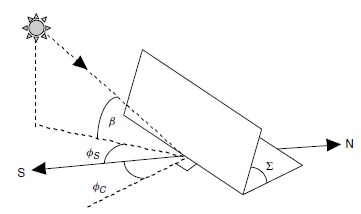
\includegraphics[scale=1]{m13}
\caption{Solar and Collector Azimuth and Altitude angles along with Collector Tilt angle [5]}
\label{figc4h14} %% to refer use, \ref{}
\end{figure}

\begin{equation}
\label{beamc3}
\cos{(\theta)}=\cos{(\beta)}\cos{(\phi_{S}-\phi_{C})}\sin{(\Sigma)}+\sin{(\beta)}\cos{(\Sigma)}
\end{equation}\\
where,\\
$ \phi_{S} $ = Azimuth angle of Sun $ (Degrees)$\\
$ \phi_{C} $ = Azimuth angle of the solar collector $ (Degrees)$\\
$ \sigma $ = Tilt angle of the solar collector $ (Degrees)$\\ 
    
\subsection{Diffuse Radiation}
\
\
\
\
The computation of diffuse radiation is complicated, as it includes the radiation scattered by the atmospheric gases, moisture etc., and also the radiation reflected from the surface which is scattered again by the atmosphere back to ground. It is fair to assume diffuse radiation to be coming with equal intensity from all directions (sky is assumed to be isotropic).
    
\begin{figure}[H]
\centering
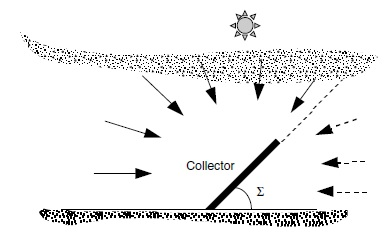
\includegraphics[scale=1]{m16}
\caption{Diffuse radiation on a collector is assumed to be proportional to the fraction of the sky that the collector "sees"  [5]}
\label{figc4h15} %% to refer use, \ref{}
\end{figure}

The eq (\ref{diff1})shows that the diffuse radiation is always dirrectly proportional to the beam radiation, where C given by the eq (\ref{diff2}) is the sky diffuse factor.

\begin{equation}
\label{diff1}
I_{DH}=CI_{B}
\end{equation}\\
where,\\
$ I_{DH} $ = Diffused portion of the radiation striking the solar collector $ (W/m^{2})$\\
$ C $ = Sky-Diffuse factor\\ 

\begin{equation}
\label{diff2}
C=0.095+0.04\sin\left[\frac{360}{365}(n-100)\right]
\end{equation}

The diffuse radiation striking the solar collector depend on the amount of sky seen by the collector. Moreover, the amount of sky seen by a solar collector is inversely proportional to its tilt angle in a sinusoidal way as given in the eq (\ref{diffc1}).

\begin{equation}
\label{diffc1}
I_{DC}=I_{DH}\left(\frac{1+\cos{(\Sigma)}}{2}\right)=CI_{B}\left(\frac{1+\cos{(\Sigma)}}{2}\right)
\end{equation}
    
    
\subsection{Reflected Radiation}
\
\
\
\
The beam and diffuse radiation incident on the ground surface, results in the their reflection off the ground surface. In the simplest model it is fair to assume that the reflected radiation from the ground surface is in equal intensity in all directions as illustrated in the Fig (\ref{figc4h16}). 
    
\begin{figure}[H]
\centering
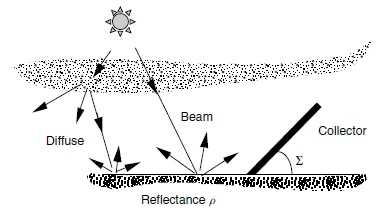
\includegraphics[scale=1]{m15}
\caption{The ground is assumed to reflect radiation with equal intensities in all directions [5]}
\label{figc4h16} %% to refer use, \ref{}
\end{figure} 

The Component reflected radiation striking the solar collector depend on the amount of ground seen by the collector. Moreover, the amount of ground seen by a solar collector is directly proportional to its tilt angle in a sinusoidal way as given in the eq (\ref{ref1}).

\begin{equation}
\label{ref1}
I_{RC}=\rho(I_{BH}+I_{DH})\left(\frac{1-\cos{(\Sigma)}}{2}\right)
\end{equation}\\
where,\\
$ I_{RC} $ = Reflected portion of the radiation striking the solar collector $ (W/m^{2})$\\
$ \rho $ = Ground Reflectance $ (Range 0.1-0.8) $\\

\subsection{Total Solar Radiation}    
\
\
\
\
The total radiation striking the solar collector is the sum of the beam, diffuse and reflected  as computed in the previous sections, it is given in the eq (\ref{totc1}).
     
\begin{equation}
\label{totc1}
I_{C}=I_{BC}+I_{DC}+I_{RC}
\end{equation}\\
where,\\
$ I_{C} $ = Total radiation incident on the solar collector $ (W/m^{2})$

A more detailed equation for the total solar radiation striking the solar collector is given by eq (\ref{totc2}), by substituting eq (\ref{beamc1},\ref{diffc1},\ref{ref1}) in eq (\ref{totc1}).

\begin{equation}
\label{totc2}
    \begin{aligned}
        I_{C}
        =Ae^{-km} \left[ \cos{(\beta)}\cos{(\phi_{S}-\phi_{C})}\sin{(\Sigma)} \\
       & + \sin{(\beta)}\cos{(\Sigma)} + C\left(\frac{1+\cos{(\Sigma)}}{2}\right) \\ \\
      & +\rho(\sin{(\beta)}+C)\left.\left(\frac{1-\cos{(\Sigma)}}{2}\right)\right]
   \end{aligned}
\end{equation}
    
   
    
\section{Radiation Equations}
\
\
\
\
The equation developed in the previous sections for the beam, diffuse and reflected radiation striking the solar collector are modified for different orientations of the Solar PV modules: Fixed Tilt, Seasonal Tilt, Single Axis Tracker and Double Axis Tracker, and presented in the following sub-sections\\
   
\subsection{Fixed Tilt Equations}
\
\
\
\ 
The equations for the beam, diffuse and reflected radiations striking the solar PV module in a fixed tilt orientation are given by eq (\ref{ft1},\ref{ft2},\ref{ft3}).

\begin{equation}
\label{ft1}
I_{BC}=I_{B}\cos{(\theta)}
\end{equation}

\begin{equation}
\label{ft2}
I_{DC}=CI_{B}\left(\frac{1+\cos{(\Sigma)}}{2}\right)
\end{equation}

\begin{equation}
\label{ft3}
I_{RC}=\rho I_{B}(\sin{(\beta)}+C)\left(\frac{1-\cos{(\Sigma)}}{2}\right)
\end{equation}


\subsection{Seasonal Tilt Equations}
\
\
\
\
The equations for the beam, diffuse and reflected radiations striking the solar PV module in a fixed tilt orientation are given by eq (\ref{st1},\ref{st2},\ref{st3}).

\begin{equation}
\label{st1}
I_{BC}=I_{B}\cos{(\theta_{\text{Tilt Type}})}
\end{equation}

\begin{equation}
\label{st2}
I_{DC}=CI_{B}\left(\frac{1+\cos{(\Sigma_{\text{Tilt Type}})}}{2}\right)
\end{equation}

\begin{equation}
\label{st3}
I_{RC}=\rho I_{B}(\sin{(\beta)}+C)\left(\frac{1-\cos{(\Sigma_{\text{Tilt Type}})}}{2}\right)
\end{equation}\\
where,\\
\textit{Tilt Type} = It can be normal, summer and winter season tilt\\


\subsection{Single-Axis Tracker Equations}
\
\
\
\
The equations for the beam, diffuse and reflected radiations striking the solar PV module in a fixed tilt orientation are given by eq (\ref{sat1},\ref{sat2},\ref{sat3}).

\begin{equation}
\label{sat1}
\Sigma_{effective}=90^{\circ}-\beta +\delta
\end{equation}

\begin{equation}
\label{sat2}
I_{BC}=I_{B}\cos{(\delta)}
\end{equation}

\begin{equation}
\label{sat3}
I_{DC}=CI_{B} \left[ \frac{1+\cos{(90^{\circ}-\beta+\delta)}}{2} \right]
\end{equation}


\begin{equation}
\label{sat4}
I_{RC}=\rho(I_{BH}+I_{DH})\left[\frac{1-\cos{(90^{\circ}-\beta+\delta)}}{2}\right]
\end{equation}


\subsection{Dual Axis Tracker Equations}
\
\
\
\
The equations for the beam, diffuse and reflected radiations striking the solar PV module in a fixed tilt orientation are given by eq (\ref{tda1},\ref{tda2},\ref{tda3}).

\begin{equation}
\label{tda1}
I_{BC}=I_{B}
\end{equation}

\begin{equation}
\label{tda2}
I_{DC}=CI_{B} \left[ \frac{1+\cos{(90^{\circ}-\beta)}}{2} \right]
\end{equation}

\begin{equation}
\label{tda3}
I_{RC}=\rho(I_{BH}+I_{DH})\left[\frac{1-\cos{(90^{\circ}-\beta)}}{2}\right]
\end{equation}

\newpage
 
\section{Power Flow through Solar PV Grid Connected System}
\
\
\
\
The Fig (\ref{PVloss}) illustrates the power flow through a solar PV system and the various losses incurred in the this system.

\begin{figure}[H]
\centering
\includegraphics[scale=0.80]{SolarPVLosses}
\caption{Flow Diagram - Power Flow and Power Losses in a Solar PV System}
\label{PVloss} %% to refer use, \ref{}
\end{figure} 

\subsection{Shading, Soiling and Incidence Angle Loss}
\
\
\
\
As seen in chapter 2, shading of PV modules leads to a reduction in power output. Shading is caused by shadows cast by near (near shading) as well as far (far shading) objects. These shadows inhibit the solar radiation from striking the PV modules causing shading and the subsequent loss in power output. To avoid shading losses the design of the PV arrays should be such that they do not cast shadow on each other, any near by objects casting shadow on the PV modules should be removed and the location of the PV system should be such that no far away objects cast shadow on the modules.\\

Soil and dust accumulated on the PV module surface reduces the amount of radiation striking the module surface causing reduction in power output. To avoid power loss due to soiling regular cleaning of PV modules has to be performed.\\

As the surface of the PV module is made out of glass there is some radiation which is reflected from the PV module surface. This results in module power loss due to the incidence angle of the beam radiation. The ASHRAE (American Society of Heating, Refrigeration, and Air Conditioning ) model for IAM is given in eq (\ref{iam}). It is a simple model as it requires only one parameter $ b_{0} $, however its accuracy reduces at higher incidence angles (Abella et al., 2003).

\begin{equation}
\label{iam}
IAM=1-b_{0} \left[ \frac{1}{ \cos {(\theta)}}-1 \right]  
\end{equation}\\
where,\\
$ IAM $ = Incidence Angle Modifier\\
$ b_{0} $ = Constant\\
$ \theta $ = Incidence Angle  $ ^{\circ}C $\\ 


From the Fig (\ref{IAM1}) it can be observed that the IAM factor reduces from 1 at 0^{\circ} to 0 at 90^{\circ}. Hence, more the incident angle more is the reflection of the radiation from the PV module surface  . To avoid IAM losses significantly single axis or double axis tracker systems are used as they always try to maintain the incidence angle to the minimum (especially the double axis tracking system). 

\begin{figure}[H]
\centering
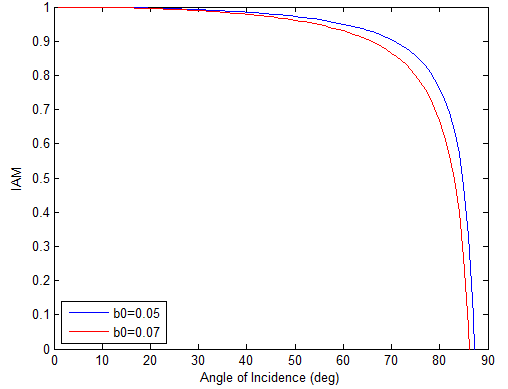
\includegraphics[scale=0.75]{IAM}
\caption{ASHRAE IAM Model}
\label{IAM1} %% to refer use, \ref{}
\end{figure} 
    
\subsection{Effect of Temperature and Irradiance on PV Module Output}
\
\
\
\
The PV module rated power given in the datasheet by the manufacturer is experimentally measured under the STC conditions of 25^{\circ}C temperature and 1000 W/m^{2} of irradiance. However, in the field the temperature and irradiance levels change continuously throughout the day and the year depending on the location of the PV system.\\

As we have seen in chapter 2, PV module power is directly proportional to solar irradiance and inversely proportional to temperature, there will be conditions when the module will generate lower than rated power (due to either high temperature or low irradiance or both), similarly thre can be conditions when the module generates more than the rated power (due to either low temperature or high irradiance or both). The eq (\ref{PVTemIrr}) gives the relationship between the actual power generated by the module.

\begin{equation}
\label{PVTemIrr}
P_{Actual}=P_{Rated}\left[1-\bigtriangledown T]\right \frac{G_{Actual}}{G_{STC}} 
\end{equation}\\
where,\\
$ P_{Actual} $ = Actual Power generated by the PV mdule $ (W) $\\
$ P_{Rated} $ = PV module rated power $ (W) $\\
$ \bigtriangledownT $ = Difference between Ambient and STC temperatures $ (^{\circ}C)$\\
$ G_{Actual} $ = Actual Solar Irradiance $ (W/m^{2}) $\\
$ G_{STC} $ = STC Solar Irradiance $ (W/m^{2}) $\\
    
\subsection{Array Mismatch and Ohmic Loss}
\
\
\
\
Mismatch losses are caused due to the differences in the outputs of individual modules in an array. The major differences between modules are of two kinds: difference in open-circuit voltage and/or difference in short-circuit current. These difference eventually cause lowering of the power output of the entire array.\\

The Fig (\ref{MisMat1}) shows two modules connected in series. In a series connection voltages of individual modules get added to give the total voltage of the string and the current flowing through all modules is the same. Hence, in this case the difference in open-circuit voltage is benign, but difference in short-circuit current is severe as the current output of the entire string is determined by the lowest current producing module, this severely reduces the the power output of the entire string. 

\begin{figure}[H]
\centering
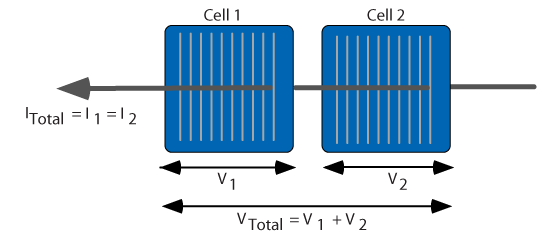
\includegraphics[scale=0.75]{Mismatch1}
\caption{Mismach in Series Connnected Modules [PV Education]}
\label{MisMat1} %% to refer use, \ref{}
\end{figure} 

Similarly in Fig (\ref{MisMat2}) shows two modules connected in parallel. In a parallel connection currents of individual modules get added to give the total current of the array and the voltage across all modules is the same. Hence, in this case the difference in  short-circuit curren is benign, but difference in open-circuit voltage is severe as the voltage output of the entire array is determined by the lowest voltage producing string, this severely reduces the the power output of the entire array. Hence, in order to reduce these array mismatch losses the manufacturing process of the modules have to be standardized so that every module is exactly similar to the other.

DC cabling is done to interconnect modules within a string, strings within an array and then to connect the PV system to the inverters. Also, AC cabling is done to connect the inverters to the transformer, and the transformer to the grid. All these cables add to the resistance of the PV system causing huge ohmic losses. Hence, in order to reduce these ohmic losses, the length of the cabling should be minimum and the cable material should be of low resistivity.

\begin{figure}[H]
\centering
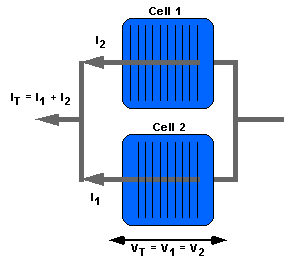
\includegraphics[scale=1]{Mismatch2}
\caption{Mismach in Parallely Connnected Modules [PV Education]}
\label{MisMat2} %% to refer use, \ref{}
\end{figure}  


    
\subsection{Inverter and Transformer Loss}   
\
\
\
\
Inverters are at the heart of the Solar PV system, the convert the DC power generated in modules to AC power which can be fed to the grid. Additionally they perform the task of maximum power point tracking, which helps in extracting maximum power from the PV modules at every temperature and irradiance condition. However, inverters are power electronic devices which are made up of high frequency switching devices; the switching devices cause loss in power due to the swtiching losses. To avoid inverter losses, a good quality inverter should be used.\\

Transformers are another indispensible part of the grid connected Solar PV systems. They step-up the voltage of the PV system output, so that the power can be transferred to the transmission lines operating at higher voltages. But, transformers consist of copper coils which result in resistive losses, and iron cores which cause iron losses. Hence, the power output to the grid from the the PV system is reduced.
   
\newpage    
   
\section{MATLAB Model Algorithm}   

The Fig (\ref{figc4halgo1} ) depicts an simplified flowchart of the algorithm which is developed for the creation of the Solar Energy Estimation Application. 
    
    
\begin{figure}[H]
\centering
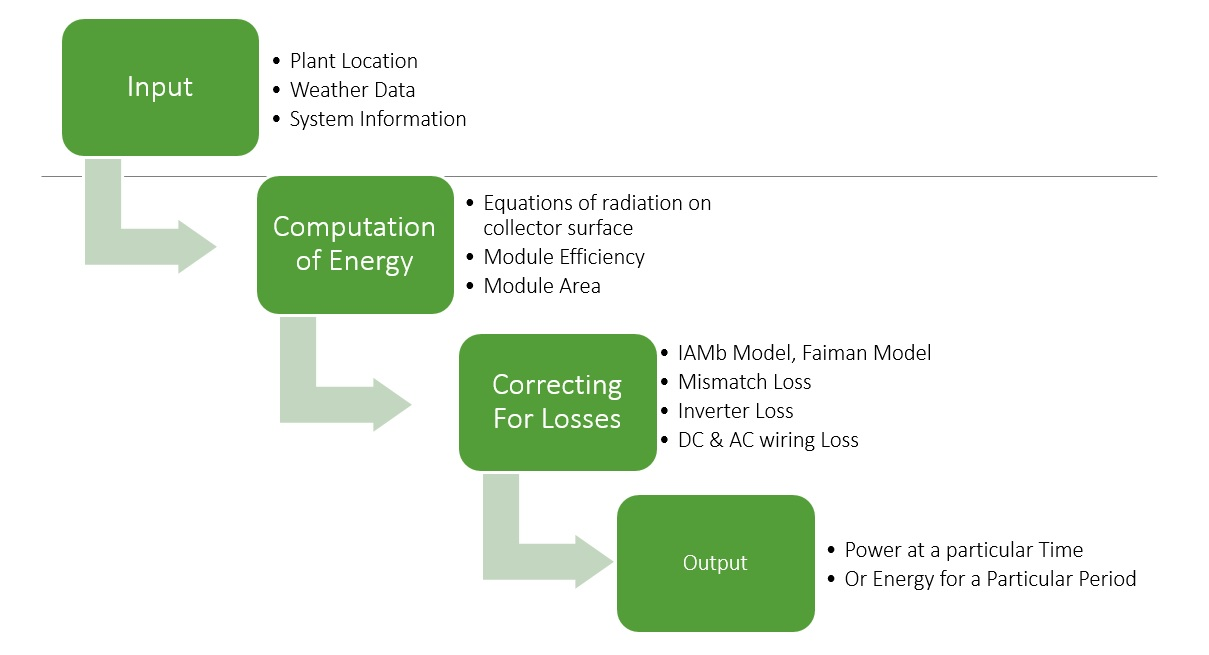
\includegraphics[scale=0.5]{SolarAppAlgorithm}
\caption{Solar Photovoltaic Energy Estimation Schematic}
\label{figc4halgo1} %% to refer use, \ref{}
\end{figure}

\newpage

Based on the theory discussed in previous sections of this chapter and the algorithm developed as illustrated in Fig (\ref{PVloss},\ref{figc4halgo1}); a GUI based application for energy estimation solar photovoltaic grid connected power plants is developed in MATLAB, the results of which are presented in the next section and the application GUIs can be found in the Appendix.
    
\section{Results of Solar Energy Estimation App}
\
\
\
\    
This section illustrates the results of energy simulation of Backbone 5MW Solar Power Plant. It is situated in Samakhiyali, Kutch, Gujarat. It has 145W Thin Film modules which are supported by a single axis east-west tracker system. Monthly enrgy output of the plant have been simulated in both the developed MATLAB application and then a comparison is done with the PVsyst simulation of the same plant.\\

The Table (\ref{SolarAppTab1}) gives the site and PV module information of the Backbone 5MW SPVP.

\begin{table}[H]
  \centering
  \caption{BackBone 5MW SPVP Information Table}
    \begin{tabular}{|l|c|}
    \hline
    \multicolumn{2}{|c|}{\textbf{BackBone 5MW SPVP}} \bigstrut\\
    \hline
    \multicolumn{2}{|c|}{\textbf{SITE INFORMATION}} \bigstrut\\
    \hline
    \textbf{LATITUDE} & 23.357 \bigstrut\\
    \hline
    \textbf{LONGITUDE} & 70.358 \bigstrut\\
    \hline
    \textbf{PLANT CAPACITY (MW)} & 5 \bigstrut\\
    \hline
    \multicolumn{2}{|c|}{\textbf{PV MODULE INFORMATION}} \bigstrut\\
    \hline
    \textbf{DESCRIPTION} & Micro-Amorphous \bigstrut\\
    \hline
    \textbf{MAKE} & NT-145AX \bigstrut\\
    \hline
    \textbf{CRYSTALLINE/THIN-FILM} & Thin-Film \bigstrut\\
    \hline
    \textbf{RATING (W)} & 145 \bigstrut\\
    \hline
    \textbf{Vmpp (V)} & 64.2 \bigstrut\\
    \hline
    \textbf{Impp (A)} & 2.26 \bigstrut\\
    \hline
    \textbf{Voc (V)} & 85.5 \bigstrut\\
    \hline
    \textbf{Isc (A)} & 2.54 \bigstrut\\
    \hline
    \textbf{TEMP COEFF OF Voc} & -0.32 \bigstrut\\
    \hline
    \textbf{TEMP COEFF OF Isc} & 0.07 \bigstrut\\
    \hline
    \textbf{TEMP COEFF OF Pmp} & -0.28 \bigstrut\\
    \hline
    \textbf{TOTAL MODULES} & 34485 \bigstrut\\
    \hline
    \textbf{LENGTH (mm)} & 1412 \bigstrut\\
    \hline
    \textbf{BREADTH (mm)} & 1112 \bigstrut\\
    \hline
    \textbf{AREA (m2)} & 1.570144 \bigstrut\\
    \hline
    \end{tabular}%
  \label{SolarAppTab1}%
\end{table}%



Figure (\ref{PVG1}) hows the graph of energy output of Backbone 5MW SPV for the year 2014 for different orientations computed using developed MATLAB application.
       
\begin{figure}[H]
\centering
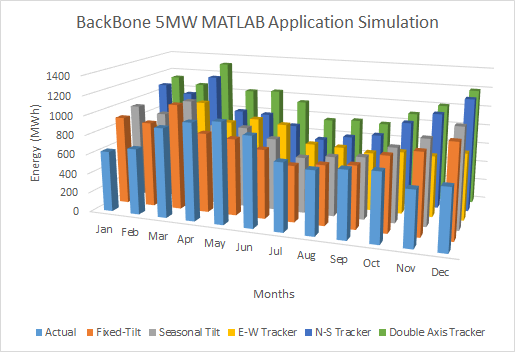
\includegraphics[scale=1]{PVresultG1}
\caption{MATLAB Application Backbone Plant month-wise energy estimation for different orientations}
\label{PVG1} %% to refer use, \ref{}
\end{figure}

In the tables FT-Fixed Tilt, ST-Seasonal Tilt, E-W-Single Axis East-West Tracker, N-S-Single Axis North-South Tracker and D-A- Double Axis Tracker\\

\begin{table}[H]
  \centering
  \caption{MATLAB BackBone Application Simulation}
    \begin{tabular}{|l|r|r|r|r|r|r|}
    \hline
    \multicolumn{7}{|c|}{\textbf{MATLAB BackBone Application Simulation}} \bigstrut\\
    \hline
       & \multicolumn{1}{l|}{\textbf{Actual }} & \multicolumn{1}{l|}{\textbf{FT}} & \multicolumn{1}{l|}{\textbf{ST}} & \multicolumn{1}{l|}{\textbf{E-W}} & \multicolumn{1}{l|}{\textbf{N-S }} & \multicolumn{1}{l|}{\textbf{D-A}} \bigstrut\\
    \hline
    \textbf{Jan} & 624 & 908 & 968 & 674 & 1095 & 1134 \bigstrut\\
    \hline
    \textbf{Feb} & 678.7 & 876 & 909 & 712 & 1014 & 1064 \bigstrut\\
    \hline
    \textbf{Mar} & 917.5 & 1087 & 1066 & 992 & 1215 & 1317 \bigstrut\\
    \hline
    \textbf{Apr} & 997.4 & 817 & 832 & 800 & 859 & 1029 \bigstrut\\
    \hline
    \textbf{May} & 1030 & 787 & 832 & 858 & 845 & 1045 \bigstrut\\
    \hline
    \textbf{Jun} & 921 & 708 & 741 & 822 & 744 & 944 \bigstrut\\
    \hline
    \textbf{Jul} & 693 & 575 & 575 & 640 & 617 & 764 \bigstrut\\
    \hline
    \textbf{Aug} & 646.9 & 613 & 613 & 633 & 670 & 782 \bigstrut\\
    \hline
    \textbf{Sep} & 682.8 & 640 & 640 & 602 & 714 & 769 \bigstrut\\
    \hline
    \textbf{Oct} & 697.7 & 763 & 763 & 641 & 871 & 902 \bigstrut\\
    \hline
    \textbf{Nov} & 562.7 & 829 & 878 & 628 & 987 & 1011 \bigstrut\\
    \hline
    \textbf{Dec} & 619.9 & 949 & 1020 & 685 & 1160 & 1191 \bigstrut\\
    \hline
    \end{tabular}%
  \label{PVresultTab1}%
\end{table}%

From Figure (\ref{PVG1}) and Table (\ref{PVresultTab1}) we see that the MATLAB application estimates the month-wise energy estimation of Backbone 5MW SPV for different orientation types. It can be seen that that there is a consistent increase in estimated energy from FT to D-A; the only outlier being the E-W estimation, this is because the tracking system has maximum and minimum azimuths of 45 and -45 respectively, and it would have been beneficial to have larger azimuths for tracking.\\

Figure (\ref{PVG2}) shows the graph of energy output of Backbone 5MW SPV for different orientations computed using PVsyst.

\begin{figure}[H]
\centering
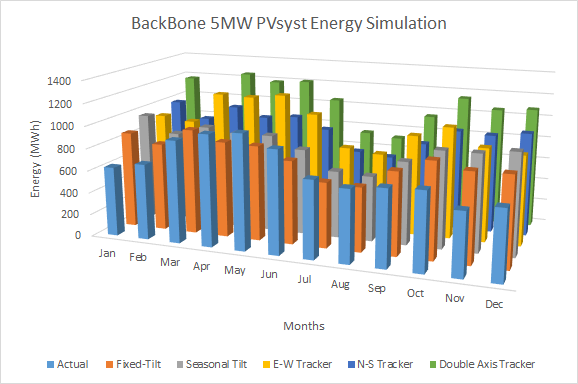
\includegraphics[scale=1]{PVresultG2}
\caption{PVsyst Backbone Plant month-wise energy estimation for different orientations}
\label{PVG2} %% to refer use, \ref{}
\end{figure}

\begin{table}[H]
  \centering
  \caption{Pvsyst BackBone Simulation Results}
    \begin{tabular}{|l|r|r|r|r|r|r|}
    \hline
    \multicolumn{7}{|c|}{\textbf{Pvsyst BackBone Simulation Results}} \bigstrut\\
    \hline
       & \multicolumn{1}{l|}{\textbf{Actual }} & \multicolumn{1}{l|}{\textbf{FT}} & \multicolumn{1}{l|}{\textbf{ST}} & \multicolumn{1}{l|}{\textbf{E-W}} & \multicolumn{1}{l|}{\textbf{N-S }} & \multicolumn{1}{l|}{\textbf{D-A}} \bigstrut\\
    \hline
    \textbf{Jan} & 624 & 866 & 967 & 908 & 985 & 1176 \bigstrut\\
    \hline
    \textbf{Feb} & 678.7 & 789 & 820 & 874 & 841 & 1023 \bigstrut\\
    \hline
    \textbf{Mar} & 917.5 & 943 & 903 & 1155 & 975 & 1250 \bigstrut\\
    \hline
    \textbf{Apr} & 997.4 & 858 & 872 & 1146 & 895 & 1189 \bigstrut\\
    \hline
    \textbf{May} & 1030 & 850 & 874 & 1183 & 923 & 1210 \bigstrut\\
    \hline
    \textbf{Jun} & 921 & 746 & 771 & 1028 & 825 & 1049 \bigstrut\\
    \hline
    \textbf{Jul} & 693 & 585 & 601 & 742 & 637 & 751 \bigstrut\\
    \hline
    \textbf{Aug} & 646.9 & 574 & 586 & 710 & 610 & 721 \bigstrut\\
    \hline
    \textbf{Sep} & 682.8 & 741 & 745 & 903 & 761 & 952 \bigstrut\\
    \hline
    \textbf{Oct} & 697.7 & 859 & 870 & 1003 & 903 & 1144 \bigstrut\\
    \hline
    \textbf{Nov} & 562.7 & 799 & 872 & 845 & 887 & 1058 \bigstrut\\
    \hline
    \textbf{Dec} & 619.9 & 804 & 911 & 808 & 929 & 1081 \bigstrut\\
    \hline
    \end{tabular}%
  \label{PVresultTab2}%
\end{table}%

From Figure (\ref{PVG2}) and Table (\ref{PVresultTab2}) we see the month-wise energy estimation of Backbone 5MW SPV for different orientation types computed using PVsyst. It can be seen that that there is a consistent increase in estimated energy from FT to D-A; here too the only outlier being the E-W estimation.\\

Table (\ref{PVresultTab3}) shows the month-wise percentage errors in the energy estimation of Backbone plant for different orientations computed using the developed MATLAB application with PVsyst being the reference.

\begin{table}[H]
  \centering
  \caption{Comparison of PVsyst and MATLAB Application}
    \begin{tabular}{|l|r|r|r|r|r|}
    \hline
    \multicolumn{6}{|c|}{\textbf{Comparison of PVsyst and MATLAB Application}} \bigstrut\\
    \hline
       & \multicolumn{1}{l|}{\textbf{FT}} & \multicolumn{1}{l|}{\textbf{ST}} & \multicolumn{1}{l|}{\textbf{E-W}} & \multicolumn{1}{l|}{\textbf{N-S }} & \multicolumn{1}{l|}{\textbf{D-A}} \bigstrut\\
    \hline
    \textbf{Jan} & -4.8 & -0.1 & 25.7 & -11.1 & 3.6 \bigstrut\\
    \hline
    \textbf{Feb} & -11.1 & -10.8 & 18.6 & -20.6 & -4 \bigstrut\\
    \hline
    \textbf{Mar} & -15.3 & -18 & 14.1 & -24.6 & -5.4 \bigstrut\\
    \hline
    \textbf{Apr} & 4.8 & 4.5 & 30.2 & 4  & 13.4 \bigstrut\\
    \hline
    \textbf{May} & 7.4 & 4.8 & 27.4 & 8.5 & 13.6 \bigstrut\\
    \hline
    \textbf{Jun} & 5.2 & 3.8 & 20 & 9.8 & 10 \bigstrut\\
    \hline
    \textbf{Jul} & 1.7 & 4.4 & 13.7 & 3.1 & -1.8 \bigstrut\\
    \hline
    \textbf{Aug} & -6.7 & -4.7 & 10.8 & -9.9 & -8.5 \bigstrut\\
    \hline
    \textbf{Sep} & 13.7 & 14.2 & 33.3 & 6.1 & 19.3 \bigstrut\\
    \hline
    \textbf{Oct} & 11.2 & 12.3 & 36.1 & 3.6 & 21.1 \bigstrut\\
    \hline
    \textbf{Nov} & -3.8 & -0.7 & 25.6 & -11.3 & 4.5 \bigstrut\\
    \hline
    \textbf{Dec} & -18.1 & -11.9 & 15.3 & -24.9 & -10.2 \bigstrut\\
    \hline
    \end{tabular}%
  \label{PVresultTab3}%
\end{table}%

From (\ref{PVresultTab3}) it is observed that the MATLAB application has underestimated the energy production on majority of the times as compared to PVsyst, also it can be seen that the errors for E-W is abnormally higher than other orientation types. If we consider absolute values of the errors the average error percentage between PVsyst and MATLAB application is 12.3\%, moreover if we do not take into account E-W values the error reduces to 9.3\%. This shows that the energy estimation model developed is computing reliable estimation of energy as it is using the site data and not the generalized data used by PVsyst.\\

Figure (\ref{PVG5}) shows a comparison between the energy estimation of the Backbone 5MW SPV, with its actual orientation of single axis east-west tracker computed using PVsyst (E-W1, associate error is Error1, in Table (\ref{PVresultTab4})) and MATLAB application (E-W2, associated error is Error2, in Table (\ref{PVresultTab4})).

\begin{figure}[H]
\centering
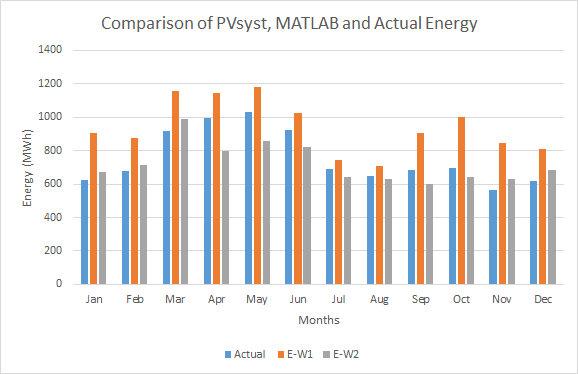
\includegraphics[scale=1]{PVresultG5}
\caption{Comparison of PVsyst, MATLAB and Actual Energy}
\label{PVG5} %% to refer use, \ref{}
\end{figure}

\begin{table}[H]
  \centering
  \caption{Comparison of PVsyst and MATLAB Application with Actual Energy}
    \begin{tabular}{|l|r|r|r|r|r|}
    \hline
    \multicolumn{6}{|c|}{\textbf{Comparison of PVsyst and MATLAB Application with Actual Energy}} \bigstrut\\
    \hline
       & \multicolumn{1}{l|}{\textbf{Actual }} & \multicolumn{1}{l|}{\textbf{E-W1}} & \multicolumn{1}{l|}{\textbf{E-W2}} & \multicolumn{1}{l|}{\textbf{Error1 \%}} & \multicolumn{1}{l|}{\textbf{Error2 \%}} \bigstrut\\
    \hline
    \textbf{Jan} & 624 & 908 & 674.3 & -45.5 & -8.1 \bigstrut\\
    \hline
    \textbf{Feb} & 678.7 & 874 & 711.5 & -28.8 & -4.8 \bigstrut\\
    \hline
    \textbf{Mar} & 917.5 & 1155 & 992.2 & -25.9 & -8.1 \bigstrut\\
    \hline
    \textbf{Apr} & 997.4 & 1146 & 799.5 & -14.9 & 19.8 \bigstrut\\
    \hline
    \textbf{May} & 1029.6 & 1183 & 858.5 & -14.9 & 16.6 \bigstrut\\
    \hline
    \textbf{Jun} & 921 & 1028 & 822.2 & -11.6 & 10.7 \bigstrut\\
    \hline
    \textbf{Jul} & 693 & 742 & 640.2 & -7.1 & 7.6 \bigstrut\\
    \hline
    \textbf{Aug} & 646.9 & 710 & 633 & -9.8 & 2.1 \bigstrut\\
    \hline
    \textbf{Sep} & 682.8 & 903 & 602.4 & -32.2 & 11.8 \bigstrut\\
    \hline
    \textbf{Oct} & 697.7 & 1003 & 640.7 & -43.7 & 8.2 \bigstrut\\
    \hline
    \textbf{Nov} & 562.7 & 845 & 628.3 & -50.2 & -11.7 \bigstrut\\
    \hline
    \textbf{Dec} & 619.9 & 808 & 684.6 & -30.3 & -10.4 \bigstrut\\
    \hline
    \end{tabular}%
  \label{PVresultTab4}%
\end{table}%

From Figure (\ref{PVG5}) and Table (\ref{PVresultTab4}) we can compare the performance of the PVsyst and MATLAB Application with actual plant data. It is observed that PVsyst overestimates the energy production with an average error percentage of 26\% (absolute values of errors), whereas the MATLAB application estimates the energy with an average error of 10\% (absolute values of errors). Hence, the developed MATLAB application performs better than PVsyst for energy estimation of the given plant.\\

Figure (\ref{PVG3}) shows a comparison between the energy estimation of the Backbone 5MW SPV, with its actual orientation of single axis east-west tracker computed the daily insolation time series file obtained from the plant (E-W3, associate error is Error3, in Table (\ref{PVresultTab5}) and using modified clear sky model (E-W4, associated error is Error4, in Table (\ref{PVresultTab5}).

\begin{table}[H]
  \centering
  \caption{ MATLAB Application Simulation Comparison of Actual, Insolation Mode and Clear Sky Model Mode}
    \begin{tabular}{|l|r|r|r|r|c|}
    \hline
    \multicolumn{6}{|c|}{\textbf{Comparison of Actual, Insolation Mode and Clear Sky Model Mode}} \bigstrut\\
    \hline
       & \multicolumn{1}{l|}{\textbf{Actual }} & \multicolumn{1}{l|}{\textbf{E-W3}} & \multicolumn{1}{l|}{\textbf{E-W4}} & \multicolumn{1}{l|}{\textbf{Error3 \%}} & \multicolumn{1}{l|}{\textbf{Error4 \%}} \bigstrut\\
    \hline
    \textbf{Jan} & 624 & 674.3 & 676.1 & -8.1 & -8.4 \bigstrut\\
    \hline
    \textbf{Feb} & 678.7 & 711.5 & 685.1 & -4.8 & -1 \bigstrut\\
    \hline
    \textbf{Mar} & 917.5 & 992.2 & 881.6 & -8.1 & 3.9 \bigstrut\\
    \hline
    \textbf{Apr} & 997.4 & 799.5 & 947.7 & 19.8 & 5 \bigstrut\\
    \hline
    \textbf{May} & 1029.6 & 858.5 & 1026.1 & 16.6 & 0.3 \bigstrut\\
    \hline
    \textbf{Jun} & 921 & 822.2 & 826.9 & 10.7 & 10.2 \bigstrut\\
    \hline
    \textbf{Jul} & 693 & 640.2 & 783.1 & 7.6 & -13 \bigstrut\\
    \hline
    \textbf{Aug} & 646.9 & 633 & 797.4 & 2.1 & -23.3 \bigstrut\\
    \hline
    \textbf{Sep} & 682.8 & 602.4 & 650.6 & 11.8 & 4.7 \bigstrut\\
    \hline
    \textbf{Oct} & 697.7 & 640.7 & 779.2 & 8.2 & -11.7 \bigstrut\\
    \hline
    \textbf{Nov} & 562.7 & 628.3 & 643.1 & -11.7 & -14.3 \bigstrut\\
    \hline
    \textbf{Dec} & 619.9 & 684.6 & 616.8 & -10.4 & 0.5 \bigstrut\\
    \hline
    \end{tabular}%
  \label{PVresultTab5}%
\end{table}%


\begin{figure}[H]
\centering
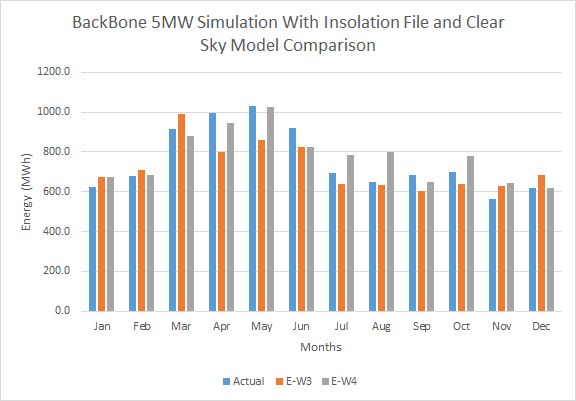
\includegraphics[scale=1]{PVresultG3}
\caption{Comparison of Insolation mode and modified Clear Sky Model mode}
\label{PVG3} %% to refer use, \ref{}
\end{figure}

From Figure (\ref{PVG3}) and Table (\ref{PVresultTab5}) we can compare two out of the three simulation modes of the MATLAB application i.e. Insolation File mode and modified clear sky model mode (SPV generation data has been correlated to the rainfall to drive clearness index). It is clearly observed that the modified clear sky mode performs better than the insolation file mode.\\

Figure (\ref{PVG4}) shows the graph of intra-day energy generation with a resolution of 15 minutes for three distinct seasonal days.

\begin{figure}[H]
\centering
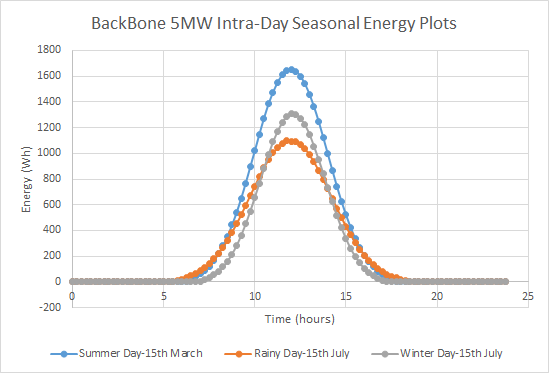
\includegraphics[scale=1]{PVresultG4}
\caption{Intra-Day Energy Estimation of Backbone Plant }
\label{PVG4} %% to refer use, \ref{}
\end{figure}

Figure (\ref{PVG4}) shows the intra-day values of energy produced by Backbone 5MW SPV at a resolution of 15 minutes. The Gaussian bell shape of the curves are due to the Gaussian disintegration of the daily insolation value received from the plant. Hence, the application has the capability to compute energy for sub-hourly resolutions.\\

\newpage

Table (\ref{PVresultTab6}) gives the plant performance of the Backbone 5MW SPV (with E-W orientation) computed by the developed MATLAB application according to the IEC Standard 61724

\begin{table}[H]
  \centering
  \caption{Plant Performance Analysis}
    \begin{tabular}{|l|r|}
    \hline
    \multicolumn{2}{|c|}{\textbf{Plant Performance Analysis}} \bigstrut\\
    \hline
    \textbf{Final Yeild (Yf)} & 1.790451 \bigstrut\\
    \hline
    \textbf{Reference Yield (Yr)} & 2.0145 \bigstrut\\
    \hline
    \textbf{Array Yeild (Ya)} & 1.902521 \bigstrut\\
    \hline
    \textbf{Temperature Corrected Reference Yeild (Yt)} & 1.990852 \bigstrut\\
    \hline
    \textbf{Thermal Capture Loss (Lct)} & 0.023647 \bigstrut\\
    \hline
    \textbf{Array Capture Loss (Lc)} & 0.111979 \bigstrut\\
    \hline
    \textbf{Miscelleneous Capture Losses (Lcm)} & 0.088332 \bigstrut\\
    \hline
    \textbf{PR} & 0.888782 \bigstrut\\
    \textbf{System Losses (Ls)} & 0.11207 \bigstrut\\
    \hline
    \hline
    \textbf{CUF} & 0.204389 \bigstrut\\
    \hline
    \textbf{Temperature Corrected PR} & 0.87847 \bigstrut\\
    \hline
    \end{tabular}%
  \label{PVresultTab6}%
\end{table}%



